

\tikzset{every picture/.style={line width=0.75pt}} %set default line width to 0.75pt        

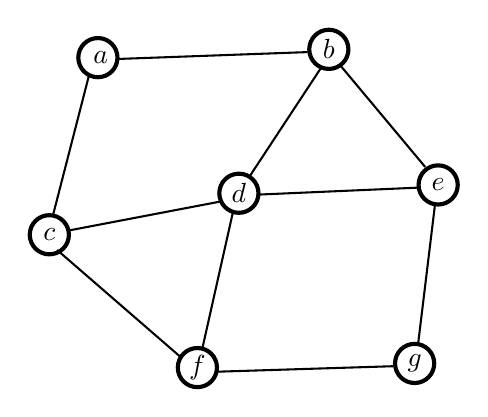
\begin{tikzpicture}[x=0.5pt,y=0.5pt,yscale=-1,xscale=1]
%uncomment if require: \path (0,319); %set diagram left start at 0, and has height of 319

%Straight Lines [id:da34511103980780045] 
\draw [color={rgb, 255:red, 0; green, 0; blue, 0 }  ,draw opacity=1 ][line width=0.75]    (269,53) -- (330,126) ;
%Straight Lines [id:da877291940114557] 
\draw [color={rgb, 255:red, 0; green, 0; blue, 0 }  ,draw opacity=1 ][line width=0.75]    (179,274) -- (307,270) ;
%Straight Lines [id:da5044796381744895] 
\draw [color={rgb, 255:red, 0; green, 0; blue, 0 }  ,draw opacity=1 ][line width=0.75]    (64,186) -- (154,264) ;
%Straight Lines [id:da8144423244977176] 
\draw [color={rgb, 255:red, 0; green, 0; blue, 0 }  ,draw opacity=1 ][line width=0.75]    (72,172) -- (182,151) ;
%Straight Lines [id:da6332136397780772] 
\draw [color={rgb, 255:red, 0; green, 0; blue, 0 }  ,draw opacity=1 ][line width=0.75]    (87,60) -- (61,161) ;
%Straight Lines [id:da39305500757559664] 
\draw [color={rgb, 255:red, 0; green, 0; blue, 0 }  ,draw opacity=1 ][line width=0.75]    (107,48) -- (245,43) ;
%Straight Lines [id:da7138338156809249] 
\draw [color={rgb, 255:red, 0; green, 0; blue, 0 }  ,draw opacity=1 ][line width=0.75]    (255,54) -- (203,133) ;
%Straight Lines [id:da014192566178230281] 
\draw [color={rgb, 255:red, 0; green, 0; blue, 0 }  ,draw opacity=1 ][line width=0.75]    (191,159) -- (169,257) ;
%Straight Lines [id:da7837916543756626] 
\draw [color={rgb, 255:red, 0; green, 0; blue, 0 }  ,draw opacity=1 ][line width=0.75]    (337,154) -- (325,253) ;
%Straight Lines [id:da9178364635401958] 
\draw [color={rgb, 255:red, 0; green, 0; blue, 0 }  ,draw opacity=1 ][line width=0.75]    (324,141) -- (209,146) ;

% Text Node
\draw  [line width=1.5]   (339.38, 139) circle [x radius= 14.15, y radius= 14.15]   ;
\draw (339.38,139) node   [align=left] {$\displaystyle e$};
% Text Node
\draw  [line width=1.5]   (93.48, 47) circle [x radius= 14.15, y radius= 14.15]   ;
\draw (87.98,47) node [anchor=west] [inner sep=0.75pt]   [align=left] {$\displaystyle a$};
% Text Node
\draw  [line width=1.5]   (260.38, 41) circle [x radius= 14.15, y radius= 14.15]   ;
\draw (260.38,41) node   [align=left] {$\displaystyle b$};
% Text Node
\draw  [line width=1.5]   (58.38, 175) circle [x radius= 14.15, y radius= 14.15]   ;
\draw (58.38,175) node   [align=left] {$\displaystyle c$};
% Text Node
\draw  [line width=1.5]   (195.38, 145) circle [x radius= 14.15, y radius= 14.15]   ;
\draw (195.38,145) node   [align=left] {$\displaystyle d$};
% Text Node
\draw  [line width=1.5]   (165.38, 271) circle [x radius= 14.15, y radius= 14.15]   ;
\draw (165.38,271) node   [align=left] {$\displaystyle f$};
% Text Node
\draw  [line width=1.5]   (322.38, 268) circle [x radius= 14.15, y radius= 14.15]   ;
\draw (322.38,268) node   [align=left] {$\displaystyle g$};


\end{tikzpicture}

